%!TEX program = xelatex
%==============================================================================
%                    JESS SULLIVAN — CV / RESUME / FUN FACTS / PROJECTS
%==============================================================================
% Compile with XeLaTeX for modern font support
% Run twice for proper cross-references
%==============================================================================

\documentclass[11pt,letterpaper]{article}

%------------------------------------------------------------------------------
% PACKAGES
%------------------------------------------------------------------------------
\PassOptionsToPackage{hyphens}{url}
\usepackage[margin=0.85in, top=0.7in, bottom=0.8in]{geometry}
\usepackage{fontspec}
\usepackage{titlesec}
\usepackage{titletoc}
\usepackage{hyperref}
\usepackage{xurl}
\setlength{\emergencystretch}{2em}
\Urlmuskip=0mu plus 1mu\relax
\usepackage{xcolor}
\usepackage{enumitem}
\usepackage{fancyhdr}
\usepackage{lastpage}
\usepackage{microtype}
\usepackage{graphicx}
\usepackage{multicol}
\usepackage{bookmark}
\usepackage{calc}
\usepackage{tikz}
\usepackage{tabularx}
\usepackage{colortbl}
\usepackage{setspace}

%------------------------------------------------------------------------------
% COLOR PALETTE
%------------------------------------------------------------------------------
\definecolor{primary}{HTML}{1a365d}
\definecolor{secondary}{HTML}{2c5282}
\definecolor{accent}{HTML}{3182ce}
\definecolor{muted}{HTML}{4a5568}
\definecolor{light}{HTML}{e2e8f0}
\definecolor{linkcolor}{HTML}{2b6cb0}

%------------------------------------------------------------------------------
% FONTS
%------------------------------------------------------------------------------
% Use Tectonic bundle filenames so builds do not depend on OS font registration.
\setmainfont{lmroman10-regular.otf}[
    BoldFont=lmroman10-bold.otf,
    ItalicFont=lmroman10-italic.otf,
    BoldItalicFont=lmroman10-bolditalic.otf
]
\setsansfont{lmsans10-regular.otf}[
    BoldFont=lmsans10-bold.otf,
    ItalicFont=lmsans10-oblique.otf,
    BoldItalicFont=lmsans10-boldoblique.otf
]
\setmonofont{lmmono10-regular.otf}[
    BoldFont=lmmonolt10-bold.otf,
    ItalicFont=lmmono10-italic.otf,
    BoldItalicFont=lmmonolt10-boldoblique.otf
]

%------------------------------------------------------------------------------
% HYPERREF CONFIGURATION
%------------------------------------------------------------------------------
\hypersetup{
    colorlinks=true,
    linkcolor=primary,
    urlcolor=linkcolor,
    citecolor=secondary,
    bookmarksnumbered=true,
    bookmarksopen=true,
    bookmarksopenlevel=1,
    pdfauthor={Jess Sullivan},
    pdftitle={Jess Sullivan — Cover Letter, Resume, Fun Facts, Projects},
    pdfsubject={Full Stack Engineer, Musician, Birdwatcher},
    pdfkeywords={DevSecOps, Machine Learning, Full Stack, HPC, Chapel, Haskell, SvelteKit},
    pdfstartview={FitH},
    pdfpagemode={UseOutlines}
}

%------------------------------------------------------------------------------
% HEADER & FOOTER
%------------------------------------------------------------------------------
\pagestyle{fancy}
\fancyhf{}
\renewcommand{\headrulewidth}{0pt}
\fancyfoot[C]{\small\color{muted} Jess Sullivan \quad$\cdot$\quad Page \thepage\ of \pageref{LastPage}}

%------------------------------------------------------------------------------
% SECTION FORMATTING
%------------------------------------------------------------------------------
\titleformat{\section}
    {\Large\bfseries\sffamily\color{primary}}
    {}
    {0em}
    {}
    [\vspace{-0.5em}\textcolor{accent}{\rule{\linewidth}{1.5pt}}]

\titleformat{\subsection}
    {\large\bfseries\sffamily\color{secondary}}
    {}
    {0em}
    {}

\titleformat{\subsubsection}
    {\normalsize\bfseries\color{muted}}
    {}
    {0em}
    {}

\titlespacing*{\section}{0pt}{1.5em}{0.8em}
\titlespacing*{\subsection}{0pt}{1em}{0.5em}
\titlespacing*{\subsubsection}{0pt}{0.8em}{0.3em}

%------------------------------------------------------------------------------
% LIST FORMATTING
%------------------------------------------------------------------------------
\setlist[itemize]{
    leftmargin=1.5em,
    itemsep=0.2em,
    parsep=0em,
    topsep=0.3em,
    label={\textcolor{accent}{\textbullet}}
}

%------------------------------------------------------------------------------
% CUSTOM COMMANDS
%------------------------------------------------------------------------------
\newcommand{\role}[2]{%
    \noindent\textbf{\color{secondary}#1} \hfill \textit{\color{muted}(#2)}\par\vspace{0.3em}
}

\newcommand{\tech}[1]{\texttt{\small\color{secondary}#1}}
\newcommand{\cvlink}[2]{\href{#1}{\color{linkcolor}#2}}

%------------------------------------------------------------------------------
% DOCUMENT START
%------------------------------------------------------------------------------
\begin{document}

%==============================================================================
% HEADER
%==============================================================================
\begin{center}
    
\begin{tikzpicture}
        \fill[primary] (0,0) rectangle (\textwidth, 0.15);
    \end{tikzpicture}
    
    \vspace{1.2em}
    
    % === HEADER IMAGE ===
    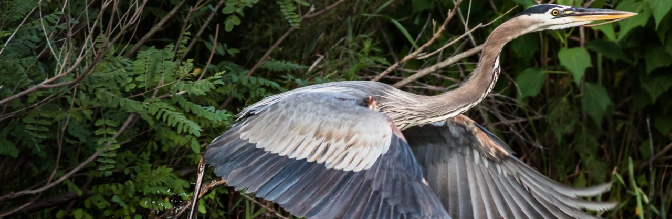
\includegraphics[width=0.85\textwidth]{header_image.png}
    
    \vspace{0.8em}
    
    {\Huge\bfseries\sffamily\color{primary} Jess Sullivan}
    
    \vspace{0.6em}
    
    {\large\itshape\color{muted} Cover Letter, Resume, Fun Facts, Projects}
    
    \vspace{1em}
    
    {\color{secondary}
    Lewiston, ME \quad$\cdot$\quad 617-795-6912 \quad$\cdot$\quad \href{mailto:jess@sulliwood.org}{jess@sulliwood.org}}
    
    \vspace{0.3em}
    
    {\small\color{secondary} \href{https://github.com/jesssullivan}{github.com/jesssullivan} \quad$\cdot$\quad \href{https://transscendsurvival.org}{transscendsurvival.org} \quad$\cdot$\quad \href{https://www.linkedin.com/in/jess-sullivan-11032a367/}{LinkedIn}}
    
    \vspace{0.5em}
    
\begin{tikzpicture}
        \fill[accent] (0,0) rectangle (\textwidth, 0.08);
    \end{tikzpicture}
\end{center}

\vspace{0.5em}

%==============================================================================
% INTRODUCTION
%==============================================================================
My name is Jess Sullivan--- I am a full stack engineer, musician and birdwatcher, currently based in Lewiston, ME. Find below a cover letter highlighting my recent and current activities and an up-to-date technical resume.

\vspace{0.5em}

%------------------------------------------------------------------------------
% NAVIGATION
%------------------------------------------------------------------------------
\begin{center}
\small\color{muted}
\hyperref[sec:resume]{\textsc{Technical Resume}} $\cdot$ 
\hyperref[sec:foss]{\textsc{Full Stack \& FOSS}} $\cdot$ 
\hyperref[sec:volunteer]{\textsc{Volunteer \& Community}} $\cdot$
\hyperref[sec:ventures]{\textsc{Ventures}} $\cdot$ 
\hyperref[sec:publications]{\textsc{Publications}} $\cdot$
\hyperref[sec:funfacts]{\textsc{Fun Facts}}
\end{center}

\vspace{0.5em}

%==============================================================================
% TECHNICAL RESUME
%==============================================================================
\section{Technical Resume}
\label{sec:resume}

%--- Computer Vision ---
\role{Computer Vision Software Engineer @ Macaulay Library}{2018--2022}

Developed \& launched \textbf{Merlin Sound ID} \& The Machine Learning Blog @ Macaulay Library. Worked on the R\&D and implementation of internal fine-grained machine learning annotation tools for audio classification. Built internal classification and model evaluation web APIs. Streamlined Macaulay Library MLOps and asset ingestion pipeline.

\vspace{0.5em}
\noindent\textit{\color{muted}My stack:}
\begin{itemize}
    \item \textbf{Model Training:} Python (\tech{tensorflow}, \tech{numpy}, \tech{pandas}, \tech{matplotlib}, \tech{JUPYTER})
    \item \textbf{Web \& training annotation stack:} \tech{Flask} \& \tech{TypeScript} (\cvlink{http://fft.js}{fft.js}, \tech{Leaflet}, \tech{React}, \tech{Vue}, \tech{Node}, \tech{Docker}, \tech{WebAssembly}, \tech{Purrr}), live demos written in \tech{React Native} and \tech{Swift}
    \item \textbf{Training and development Infra:} Project managed in Confluence + BitBucket, hosting on EC2 \& Heroku
\end{itemize}

\vspace{0.8em}

%--- Fab Lab ---
\role{Fabrication Laboratory Manager for the Landscape Architecture Makerspace @ Cornell CALS}{2021--2022}

Developed and taught rapid fabrication curricula for DLA students and faculty.

\vspace{0.5em}
\noindent\textit{\color{muted}My stack:}
\begin{itemize}
    \item \tech{OpenSCAD} \& \tech{Fusion 360}; \tech{Inkscape} for vector work. Some tiler development with TAs in \tech{C++}.
    \item Project management in GitHub \& Linear. Built a small Discord ticketing system and OBS printer monitoring system.
\end{itemize}

\vspace{0.8em}

%--- Systems Analyst ---
\role{Systems Analyst (DevSecOps) @ Bates College}{2024--Present}

Building and maintaining reliable, scalable enterprise systems directly supporting staff, faculty and the technical ILS team. Responsibilities include the maintenance and modernization of legacy systems; the development of bespoke Ansible extensions, roles, and plugins; 24/7 availability for CVE mitigation; SAML and application interoperability integration work; Open Telemetry and reporting development; the development of CI/CD pipelines (extensive work in GitLab AutoDevOps, OpenTofu and RKE2 + Rancher clusters) as well as leading IaC adoption across the College. I enjoy a fair amount of autonomy, and can be found wriggling across a wide variety of languages, projects and epics throughout any given week.

\subsubsection{Noteworthy projects include:}
\begin{itemize}
    \item Developed high performance orchestrator and instrumentation tooling for degree management and degree auditing software in \tech{Haskell} + \tech{Python} (QuickCheck, Cabal, podman-compose for development, FPM for packaging and autodevops for CI/CD); uplifted ``unautomatable'' 1980s morris-worm era code unique to higher ed into a verifiable, traceable, k8s friendly workload
    \item Overhauled and completely automated the lifecycle of our event management system (extensive development in \tech{C\#}, \tech{Go}, \tech{Ansible})
    \item Led adoption of horizontally scalable \tech{Apache Solr} instances for multiple public and private indexing and search applications
    \item Led adoption and built out numerous internal ACME-first certificate management and DNS libraries, templates and tooling
    \item Extensive work and peer education around enterprise secret management patterns and SAML at the college. Developed numerous SAML integrations, LTI integrations, Shibboleth and led adoption of \tech{KeePassXC} as part of a declarative Ansible workflow.
\end{itemize}

%==============================================================================
\newpage
%==============================================================================

%==============================================================================
% FULL STACK & FOSS
%==============================================================================
\section{Full Stack Contracting and FOSS}
\label{sec:foss}

Long term committer, member and supporter of numerous organizations including the \textbf{Rocky Enterprise Linux Foundation}, \cvlink{https://github.com/rspamd/rspamd/pull/5923}{\textbf{rspamd}}, \textbf{Chapel-lang}, \cvlink{https://github.com/numtide/nix-vm-test/pull/172}{\textbf{numtide}/nix-vm-test}, \cvlink{https://github.com/manaflow-ai/cmux/pull/1877}{\textbf{manaflow-ai}/cmux}, \cvlink{https://github.com/diku-dk/futhark/pull/2365}{\textbf{diku-dk}/Futhark}, \textbf{Liqo}, the \textbf{Apache Foundation}, \cvlink{https://github.com/caddyserver/xcaddy/pull/238}{\textbf{xCaddy}}, \textbf{libdns}, \tech{Skeleton UI}, \textbf{Klipper}, \textbf{Joplin}, \textbf{FFT.js}, \textbf{KeePassXC}, and \tech{svelte-superforms}, along with the creation of numerous FOSS automation tools and GIS utilities.

\begin{itemize}
    \item Extensive technical work with startups including \textbf{Dover Micro} (2017) and \textbf{Adaptive Motorsport} (2018)
    \item Developed web GIS tools used by the \textbf{National Park Service}, \textbf{Foundation for Healthy Communities}, \textbf{GPRED}, the \textbf{Northern Border Regional Commission}, presented at the 2019 \textbf{AAG Annual Meeting} in Washington, DC (\S\ref{sec:publications})
    \item \textbf{Machine Learning} with \textbf{MushroomObserver.org} and \textbf{Visipedia:} Collaborated on the development and adoption of fine-grained image classification models among crowd-sourced community science niches
    \item \textbf{Current package work:} \cvlink{https://github.com/Jesssullivan/scheduling-bridge/pull/135}{\tech{scheduling-bridge}}, \cvlink{https://github.com/Jesssullivan/scheduling-kit/pull/94}{\tech{scheduling-kit}}, \cvlink{https://github.com/tinyland-inc/tinyland-auth}{\tech{tinyland-auth}} TOTP/RBAC, \cvlink{https://github.com/Jesssullivan/tummycrypt}{\tech{tummycrypt}} (\cvlink{https://github.com/Jesssullivan/tummycrypt/pull/356}{TCFS proof}), and \cvlink{https://github.com/tinyland-inc/bazel-registry/pull/42}{Tinyland Bazel registry releases}.
    \item \textbf{Expanded client list} on request. Current clients include the entire business stack for \cvlink{https://MassageIthaca.com}{\textbf{MassageIthaca.com}} (grown through four business expansions over 3 years!), \textbf{Rossel \& Co}, Tetrahedron Services, R\&D for TimberBuddy hydraulic sawmill systems, many more.
\end{itemize}

\vspace{0.8em}

\noindent\textit{\color{muted}My current stack:}
\begin{itemize}
    \item \textbf{Web:} \tech{SvelteKit}, Runes, TS7, Vite 8 (Rolldown). I am deeply embedded in SvelteKit and have developed a broad library of packages and expertise ranging from fingerprinting, mapping, authentication, scheduling, horizontal data scalability and telemetry. This site/CV lives in \cvlink{https://github.com/Jesssullivan/jesssullivan.github.io}{\tech{jesssullivan.github.io}}.
    \item \textbf{HPC} and performance oriented code written in \textbf{Chapel} and increasingly \textbf{Haskell}; \textbf{TensorFlow}, \textbf{pandas}, NUMA-aware horizontal parallelism, and realtime evaluation/inference from earlier ML production work.
\end{itemize}

\vspace{0.5em}

\noindent\textit{\color{muted}Research:}

\begin{itemize}
    \item \textbf{Reverse Engineering \& Binary Analysis:} \tech{GhidraScript}, \tech{Frida}, \tech{ILSpy}, Mitre \cvlink{https://github.com/Jesssullivan/caldera}{Caldera}, \tech{Zig} --- firmware RE and \cvlink{https://github.com/Jesssullivan/hiberpower-ntfs/pull/1}{NVMe XRAM recovery} (see \S\ref{sec:publications}).
    \item \textbf{Author of numerous Zig capability libraries} with C ABI surfaces and cross-platform builds: \cvlink{https://github.com/Jesssullivan/zig-crypto}{\tech{zig-crypto}} (\cvlink{https://transscendsurvival.org/zig-crypto/}{docs}), \cvlink{https://github.com/Jesssullivan/zig-notify}{\tech{zig-notify}} (\cvlink{https://transscendsurvival.org/zig-notify/}{docs}), \cvlink{https://github.com/Jesssullivan/zig-keychain}{\tech{zig-keychain}} (\cvlink{https://transscendsurvival.org/zig-keychain/}{docs}), and \cvlink{https://github.com/Jesssullivan/zig-ctap2}{\tech{zig-ctap2}} (\cvlink{https://transscendsurvival.org/zig-ctap2/}{docs}).
    \item \cvlink{https://github.com/tinyland-inc/linux-xr}{\textbf{linux-xr}} --- Rocky Linux 10 RPM kernel lane carrying XR display patches and \cvlink{https://github.com/tinyland-inc/linux-xr/pull/66}{Dirty Frag security backports}. Backported \textbf{CVE-2026-31431}, \textbf{CVE-2026-43284}, and \textbf{CVE-2026-43500} into 6.1.y ahead of public disclosure.
    \item \textbf{Heterogeneous Compute:} \tech{WebGPU}, \tech{Futhark} (GPU-targeting functional language) --- exploring GPU-accelerated workloads and deeper WASM integration for inference pipelines.
    \item \textbf{Functional Programming:} ESDT Monads and pixelwise classification research (\cvlink{https://github.com/Jesssullivan/pixelwise-research}{pixelwise-research}). \tech{Rust} (SIMD), \tech{Nix} (build systems). With years of friendly pressure from my friend Lena Berlin (Innovation @ Analog Devices, SHARC, Farmblox), 2026 may be my first year of learning Rust in earnest.
\end{itemize}

%==============================================================================
% VOLUNTEER & COMMUNITY
%==============================================================================
\section{Volunteer, Community Involvement and Board Positions}
\label{sec:volunteer}

\role{First Fellow @ the D\&M Makerspace at Plymouth State University (``PSU'')}{2017--2020}

\begin{itemize}
    \item Taught \textbf{Advanced GIS Programming} \& \textbf{Intro to Electromechanics} at PSU
    \item Coordinated the development and manufacture of ventilators, shields and positive pressure masks with makerspaces throughout New England at the onset of the COVID-19 pandemic; worked with the Artisans Asylum (Cambridge, MA) and the NH hospital system to deliver 3d printed and lasercut medical supplies, used and distributed throughout the state.
\end{itemize}

\vspace{0.5em}

\role{Membership Chair and 3d Printing Captain of the Ithaca Generator (``IG'')}{2020--2022}

\begin{itemize}
    \item Led IG, a local 501(c)3 non-profit Makerspace through a period of rapid growth, profitable outreach and massive educational expansion
    \item Coached hundreds of students through my popular, portable \& public-facing ``\textbf{Fusion 360 for 3d printing}'' class series throughout New York
\end{itemize}

%==============================================================================
\newpage
%==============================================================================

%==============================================================================
% VENTURES
%==============================================================================
\section{Ventures}
\label{sec:ventures}

\role{Columbari.us LLC}{2017--2021}

Independent contractor / contributor business while in the GIS \& ML space. Fully insured and registered in both NH and NY. Structured solely to better negotiate contracts with UNH, NH municipal works and later Cornell.

\vspace{0.8em}

\role{Moonlight Coworking LLC}{2021--2024}

Formed in NY to raise capital and interest in a for-profit hackerspace with a focus on mathematics and high performance computing alongside my nonprofit work leading the Ithaca Generator; shelved due to move to Maine.

\vspace{0.8em}

\role{Tinyland, Inc (\cvlink{https://github.com/tinyland-inc}{github.com/tinyland-inc})}{2024--present}

Agent orchestration platform for semiautonomous infrastructure lifecycle management in higher education. Bootstrapped and in stealth; source-available where appropriate. Infrastructure flywheel work spans \cvlink{https://github.com/tinyland-inc/GloriousFlywheel}{GloriousFlywheel} (\cvlink{https://tinyland-inc.github.io/GloriousFlywheel/}{docs}), \cvlink{https://github.com/tinyland-inc/blahaj}{blahaj}, \cvlink{https://github.com/tinyland-inc/lab}{lab}, \cvlink{https://github.com/tinyland-inc/tinyland-auth}{tinyland-auth}, and the \cvlink{https://github.com/tinyland-inc/bazel-registry/pull/42}{Tinyland Bazel registry}.

%==============================================================================
\newpage
%==============================================================================

%==============================================================================
% PUBLICATIONS
%==============================================================================
\section{Publications}
\label{sec:publications}

Reitsma, L.R., Burns, C., \& \textbf{Sullivan, J.} (2019). \textit{Poecile atricapillus} (Black-capped Chickadee) Feeding \textit{Catharus guttatus} (Hermit Thrush) Nestlings. \textit{Northeastern Naturalist}, 26(2). \cvlink{https://doi.org/10.1656/045.026.0213}{doi:10.1656/045.026.0213}

\vspace{0.3em}
\noindent First recorded instance of interspecific parental feeding between these two species, documented at Plymouth State University. Field observation and video documentation of a Black-capped Chickadee provisioning Hermit Thrush nestlings over sustained periods, resulting in successful fledging.

\vspace{0.8em}

\textbf{Sullivan, J.} (2026). Recovering Write-Protected NVMe SSDs Through USB Bridge XRAM Injection: Bypassing the ASMedia ASM2362 Firmware Opcode Whitelist. \cvlink{https://transscendsurvival.org/papers/recovery-paper.pdf}{recovery-paper.pdf}

\vspace{0.3em}
\noindent Novel technique for recovering firmware write-protected NVMe SSDs over USB by injecting NVMe Submission Queue entries directly into the ASMedia ASM2362 bridge controller's internal XRAM via vendor SCSI commands, bypassing the bridge's opcode whitelist. Demonstrated successful recovery of a Phison PS5012-E12 based SSD from permanent silent-write-failure mode using Sanitize Block Erase via XRAM injection and PCIe TLP doorbell signaling.

\vspace{1em}
\subsection{Presentations}

\textbf{Sullivan, J.} (2019). Web GIS: Telling Stories \& Solving Problems. \textit{Association of American Geographers (AAG) Annual Meeting}, Washington, DC.

\vspace{0.3em}
\noindent Presented community-driven GIS mapping and Photovoice methods for youth recreation access in New Hampshire, alongside avian field research tools built with R, Shiny, and GDAL for KML/CSV/SHP data conversion and centroid analysis of banded bird territories. Work conducted in collaboration with the National Park Service, Foundation for Healthy Communities, GPRED, and Northern Border Regional Commission.

%==============================================================================
\newpage
%==============================================================================

%==============================================================================
% FUN FACTS
%==============================================================================
\section{Some More Fun Facts About Me and My Eclectic Work History}
\label{sec:funfacts}

\subsection{Professional Photography}

Commercial photography business--- paid my way through my undergraduate degree!

\begin{itemize}
    \item I cut my teeth professionally with the \textbf{world renowned aerial photographer Alex Maclean} and with \textbf{Mike Nyman Wedding Photography} prior to going into business as \textbf{J.S. Event Photography}.
    \item \textbf{I wrote} (and taught for three years!) \textbf{the youth photography curriculum} at the \textbf{Joppa Flats} and \textbf{Drumlin Farm} Mass Audubon Wildlife sanctuaries, \textbf{programs still going strong} to this day!
    \item Some public clients and superlatives of this chapter of my life included \textbf{extensive} work for the \textbf{corporate branding offices} of the \textbf{YMCA}, The \textbf{Watertown Savings Bank}, photography and videography for the \textbf{YCCA} youth programs, \textbf{FUUSN} and serving as the \textbf{Staff Photographer for MCCS @ PSU} among others.
    \item My work has been featured, displayed and sold at numerous photo shows, venues and art sales throughout New England, including many shows with \textbf{Celebrate Newton}, The \textbf{Newton Public Library}, The \textbf{Pease Public Library} in NH, \textbf{Newtonville Cinema}, \textbf{Just Next Door Card Shop}, The \textbf{Newton Camera Club}, \textbf{Broadmoor Wildlife Sanctuary}, featured in the \textbf{Newton Tab newspaper} and many others.
    \item I did much of my own printing with a heavily modified inkjet printer. \textbf{Was completely burnt out} from photography by the end of 2017 or thereabouts, sold all my gear by the end of college.
\end{itemize}

\vspace{0.8em}

\subsection{Bartending, Music and Bagels}

I am a multiinstrumentalist and am usually practicing guitar or organ when I am not writing code or looking for birds outside.

\begin{itemize}
    \item I have played guitar pretty seriously for over 20 years; I currently play a custom 9 string electric guitar made for me in NH and a 12 string acoustic.
    \item I've been playing the piano for over 25 years; my keyboard playing these days is primarily on my wacky rotary Yamaha organ.
\end{itemize}

I enjoy bartending, baking and music as social hobbies, adjacent to my oddball enthusiasm for esoteric spirits, distilling technologies, gluten and rock \& roll. As such, I've held a number of delightful evening bartender \& bakery positions:

\begin{itemize}
    \item I was an evening bartender and event organizer at \textbf{Modern Alchemy Game Bar} in Ithaca. I organized and hosted monthly Goth Nights, art shows and many other private functions for various organizations I've been affiliated with in this cozy board game bar.
    \item I was a bartender at \textbf{The Downstairs} Listening room \& Tavern as well as at \textbf{the Watershed} in New York.
    \item I was a casual Bagel Baker at Tandem Bagel Co in Northampton MA throughout the Spring of 2024. I made many terrific friends here and learned a great deal about baking professionally.
\end{itemize}

\vspace{1.5em}

\begin{center}
    \textcolor{muted}{\rule{0.4\textwidth}{0.5pt}}
    
    \vspace{0.8em}
    
    {\large\itshape\color{muted} If there were no computers I'd probably be a baker, a minstrel or a bard.}
\end{center}

%==============================================================================
% END
%==============================================================================

\vfill

\begin{center}
    
\begin{tikzpicture}
        \fill[primary] (0,0) rectangle (\textwidth, 0.1);
    \end{tikzpicture}
\end{center}

\end{document}
